\section{Model Exercise 1-1 (05): Swelling of clay}
\label{sec:mex05}
%------------------------------------------------------------------------------
\Authors{Amir Sattari, Keita Yoshioka, Mattias Nest}
%------------------------------------------------------------------------------
Model Exercise (MEX 1-1) investigates the developed pathways during the swelling progress in Opalinus clay stone material. The experimental results from developed swelling pressure in constrained swelling test in Oedometer test as well as heaving in unconstrained condition will be compared to the numerical results. 

\subsection{Experimental set-up}
%------------------------------------------------------------------------------
the constrained swelling tests using the Oedometer tests on Opalinus clay stone is conducted by \cite{Peronetal2009}.The shale formation is excavated form Mont-Terri Underground Laboratory in Switzerland. With a load cell below the setup as shown in Fig. \ref{fig:Amir_ME5_Swelling_Setup}, the swelling pressure with a resolution of 5 kPa is carried out. Fig. \ref{fig:Amir_ME5_Swelling_Constrained} shows the developed swelling pressure with time in two different shale  and one sandy claystones. 

\begin{figure}[!ht]
\centering
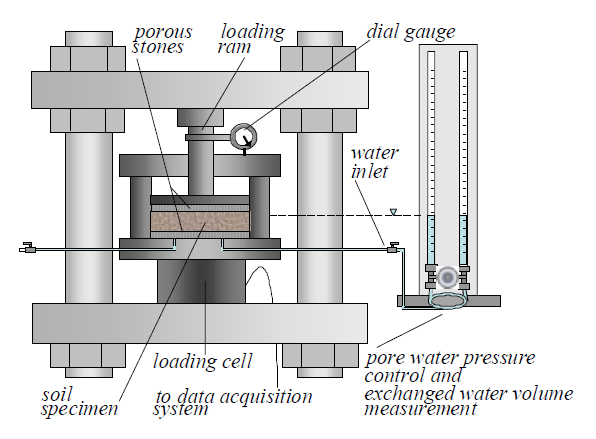
\includegraphics[width=0.75\textwidth]{figures/Amir_ME5_Swelling_Setup.png}
\caption{The Oedometer test setup for constrained swelling pressure in Opalinus clay samples \cite{Peronetal2009}}
\label{fig:Amir_ME5_Swelling_Setup}
\end{figure}

\begin{figure}[!ht]
\centering
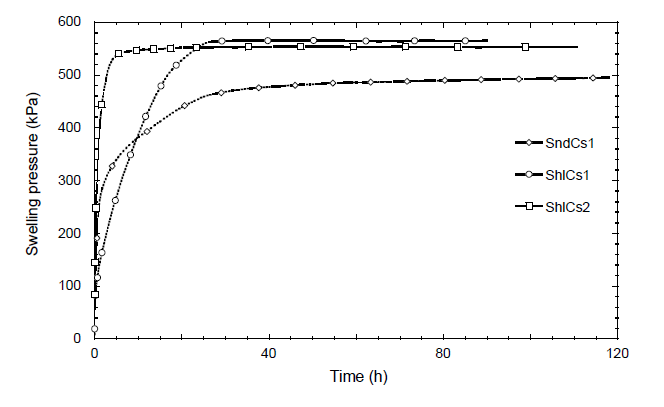
\includegraphics[width=0.75\textwidth]{figures/Amir_ME5_Swelling_Constrained.png}
\caption{The development of swelling pressure in Opalinus Clay vs. time \cite{Peronetal2009}}
\label{fig:Amir_ME5_Swelling_Constrained}
\end{figure}

%------------------------------------------------------------------------------
\subsection{Model approach}

The simulation results from each of the model methods, discrete element method (DEM), lattice element method (LEM) and phase field method (PFM) are described and the accuracy of numerical results for modeling the swelling pressure and heaving under constrained and unconstrained selling tests are investigated.

\subsubsection*{Discrete element model}

\todo[inline]{[IfG] Please add DEM results}

\subsubsection*{Lattice element model}

The developed lattice element model is base on expansion of elements to simulate the swelling in clay stone, similar approach for shrinkage modeling is used in DEM \cite{Simaetal2013}. The swelling coefficient is trained according to experimental data to determine the heave and swelling pressure applied on top plate. 

\todo[inline]{[CAU] Please add LEM results}

\subsubsection*{Finite element approach: Variational phase-field}

\todo[inline]{[UFZ](KY) Please add FEM-VPF results}

%------------------------------------------------------------------------------
\subsection{Results and discussion}